\providecommand{\path}{..}

\makeatletter
\def\input@path{{\path/}{.}}
\makeatother

\documentclass[main.tex]{subfiles}
\begin{document}
\section{Electrical improvements}

In the process of setting up and running experiments, various electrical concerns were found - some pre-emptively, and others post-hoc. The robot uses a Lithium Polymer battery, a type for which electrical mistakes can be catastrophic\footnote{An example being the newsworthy \cite{bbc-samsung-explosion} issues with the Galaxy Note 7} - making it important to avoid mistakes, and if they are made, preventing them being repeated. In line with the risk assessment, a fire-safe battery storage bag was purchased for the project.

The simplest of these was the connection of the battery to the robot, which was made using an unpolarized and uninsulated connector, show in \cref{fig:connectors}. A similar connector was used to charge the robot. Misconnecting either of these would result in outcomes ranging from a destroyed microcontroller to an exploding battery. Having exposed connections on loose flexible wires entails similar risk. These were replaced with JST RCY connectors.

Another issue with LiPo batteries, thankfully without safety ramifications, is over-discharging them. The protection circuits within the battery cause it to enter a `sleep mode' \cite{lipo-sleep-mode}, from which it cannot be restored without a more advanced charger. After being caught out by the first battery entering this state, a battery monitor was purchased (visible in \cref{fig:robot-back}), which gives a voltage readout, and an audible alarm whenever the battery needs charging.

\begin{figure}
	\centering
	\includegraphics[width=\linewidth]{figures/electronic-back.png}
	\caption{The back of the robot}
	\label{fig:robot-back}
	\medskip
	\small
	Showing the battery monitor, a button to interact with the embedded software, and velcro battery strap
	(replacing previous duct tape).
\end{figure}

\begin{figure}
	\begin{minipage}[t]{0.45\linewidth}
		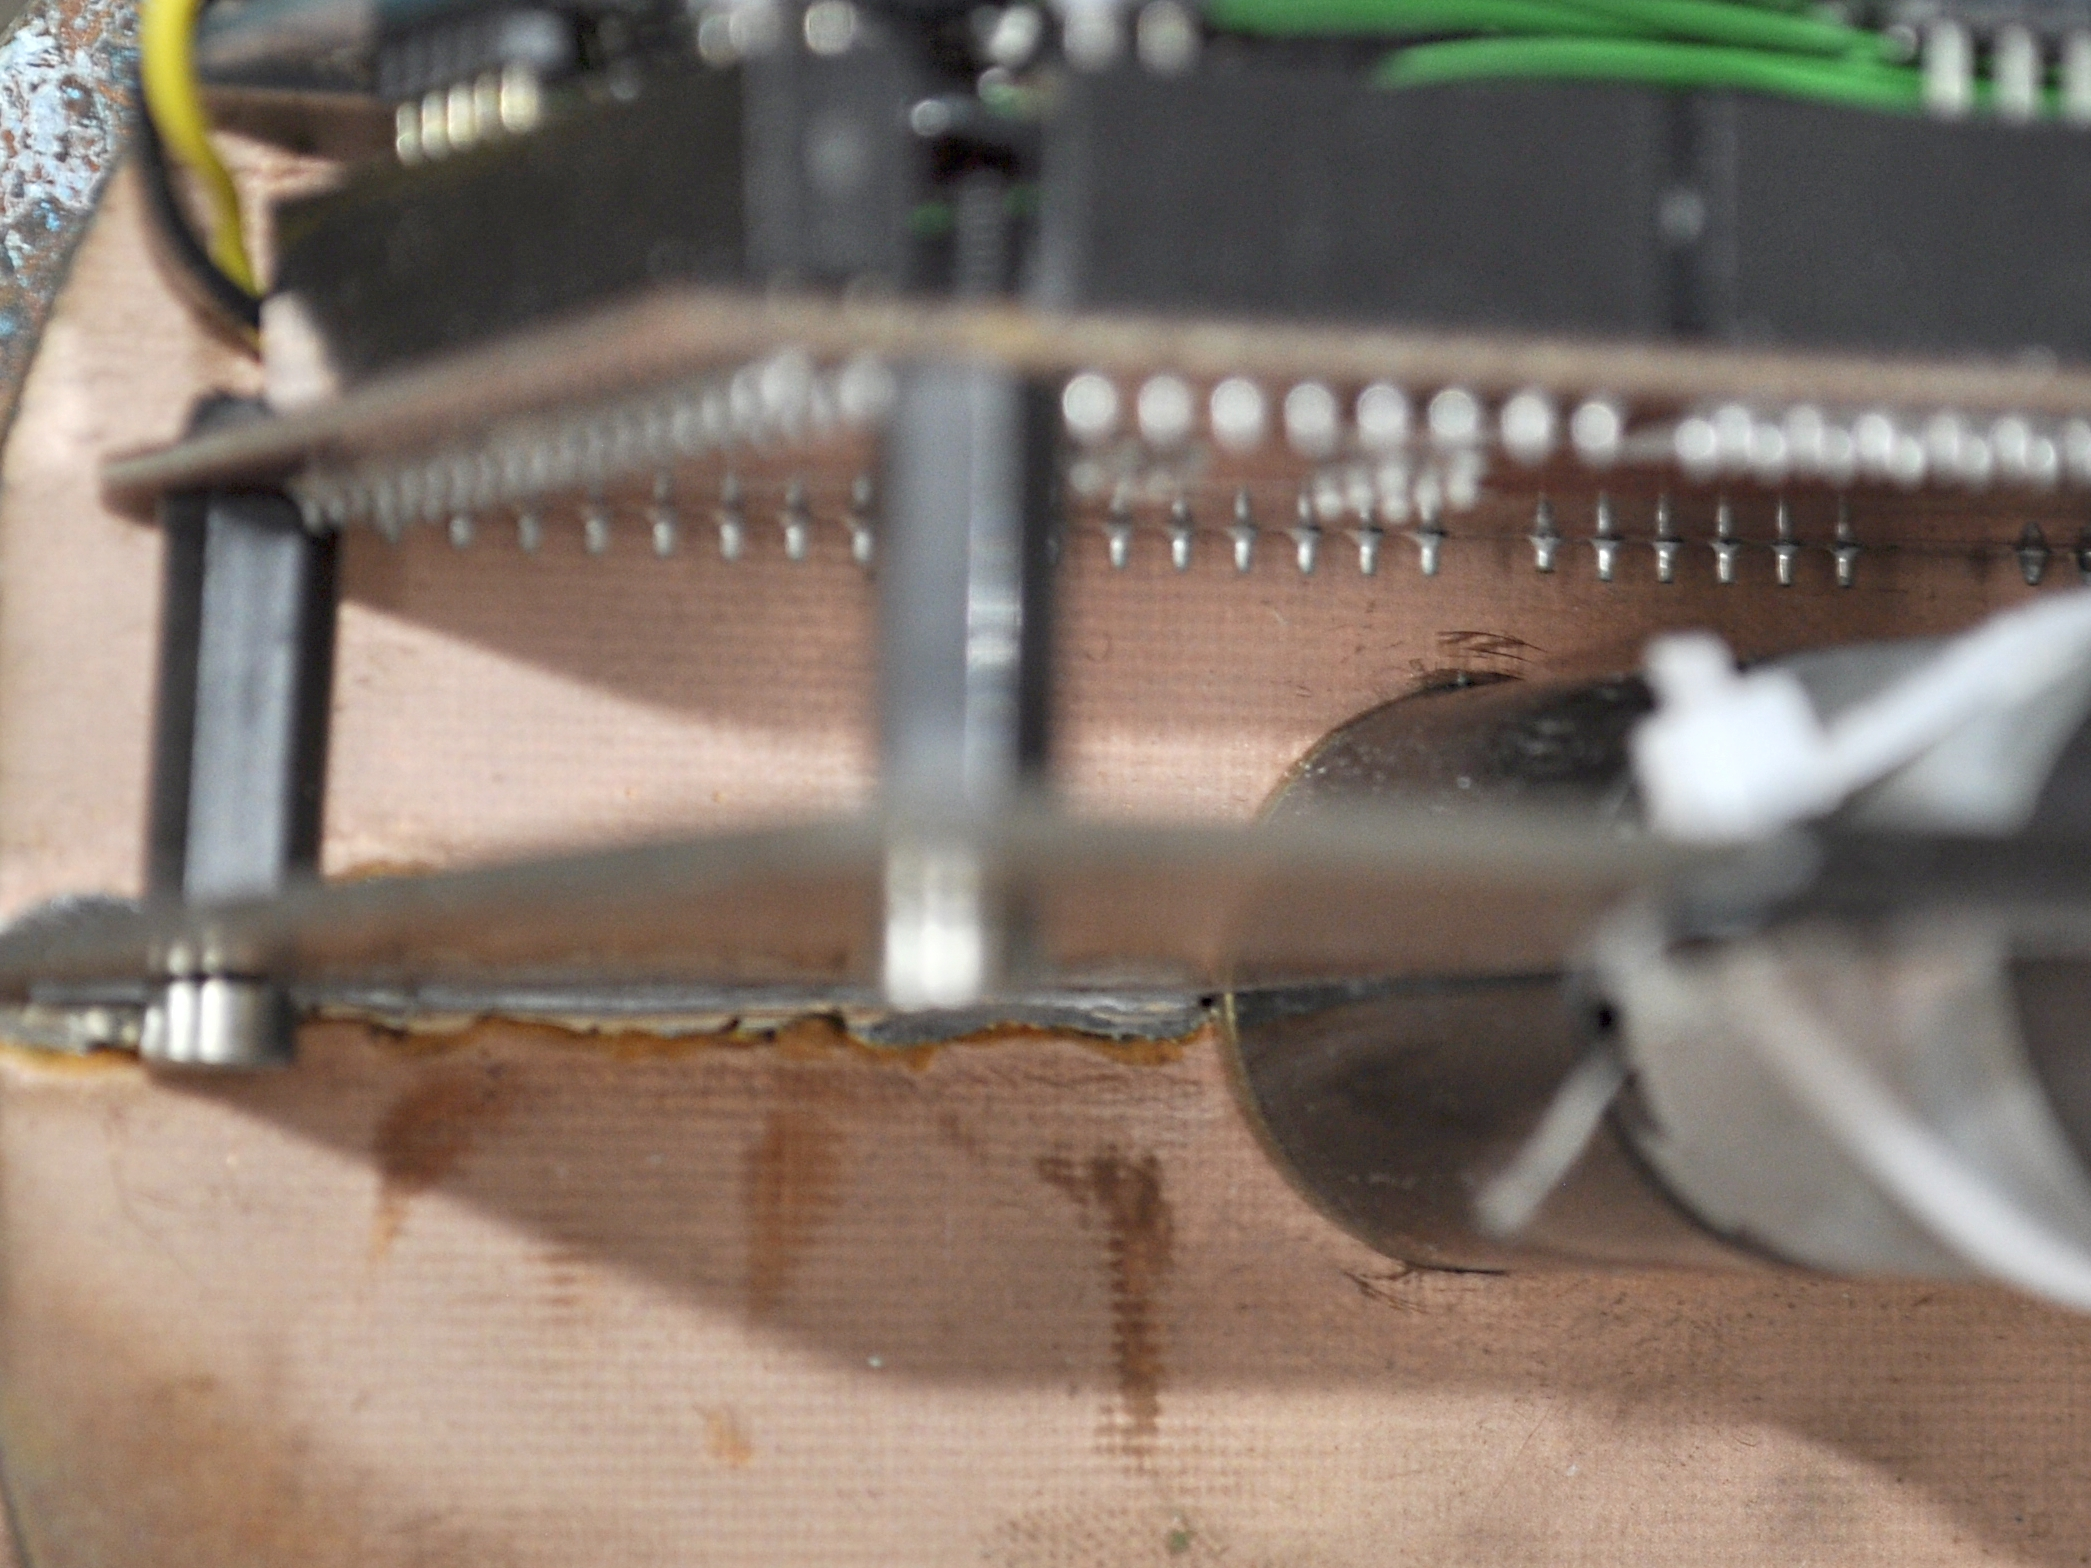
\includegraphics[width=\linewidth]{figures/standoffs.jpg}
		\caption{Clearance under the controller}
		\label{fig:clearance}
		\medskip
		\small
		The black nylon standoffs replace the old metal screws. There is now a
		clear gap between the motor (right) and the pins, preventing shorts.
	\end{minipage}
	\hfill
	\begin{minipage}[t]{0.45\linewidth}
		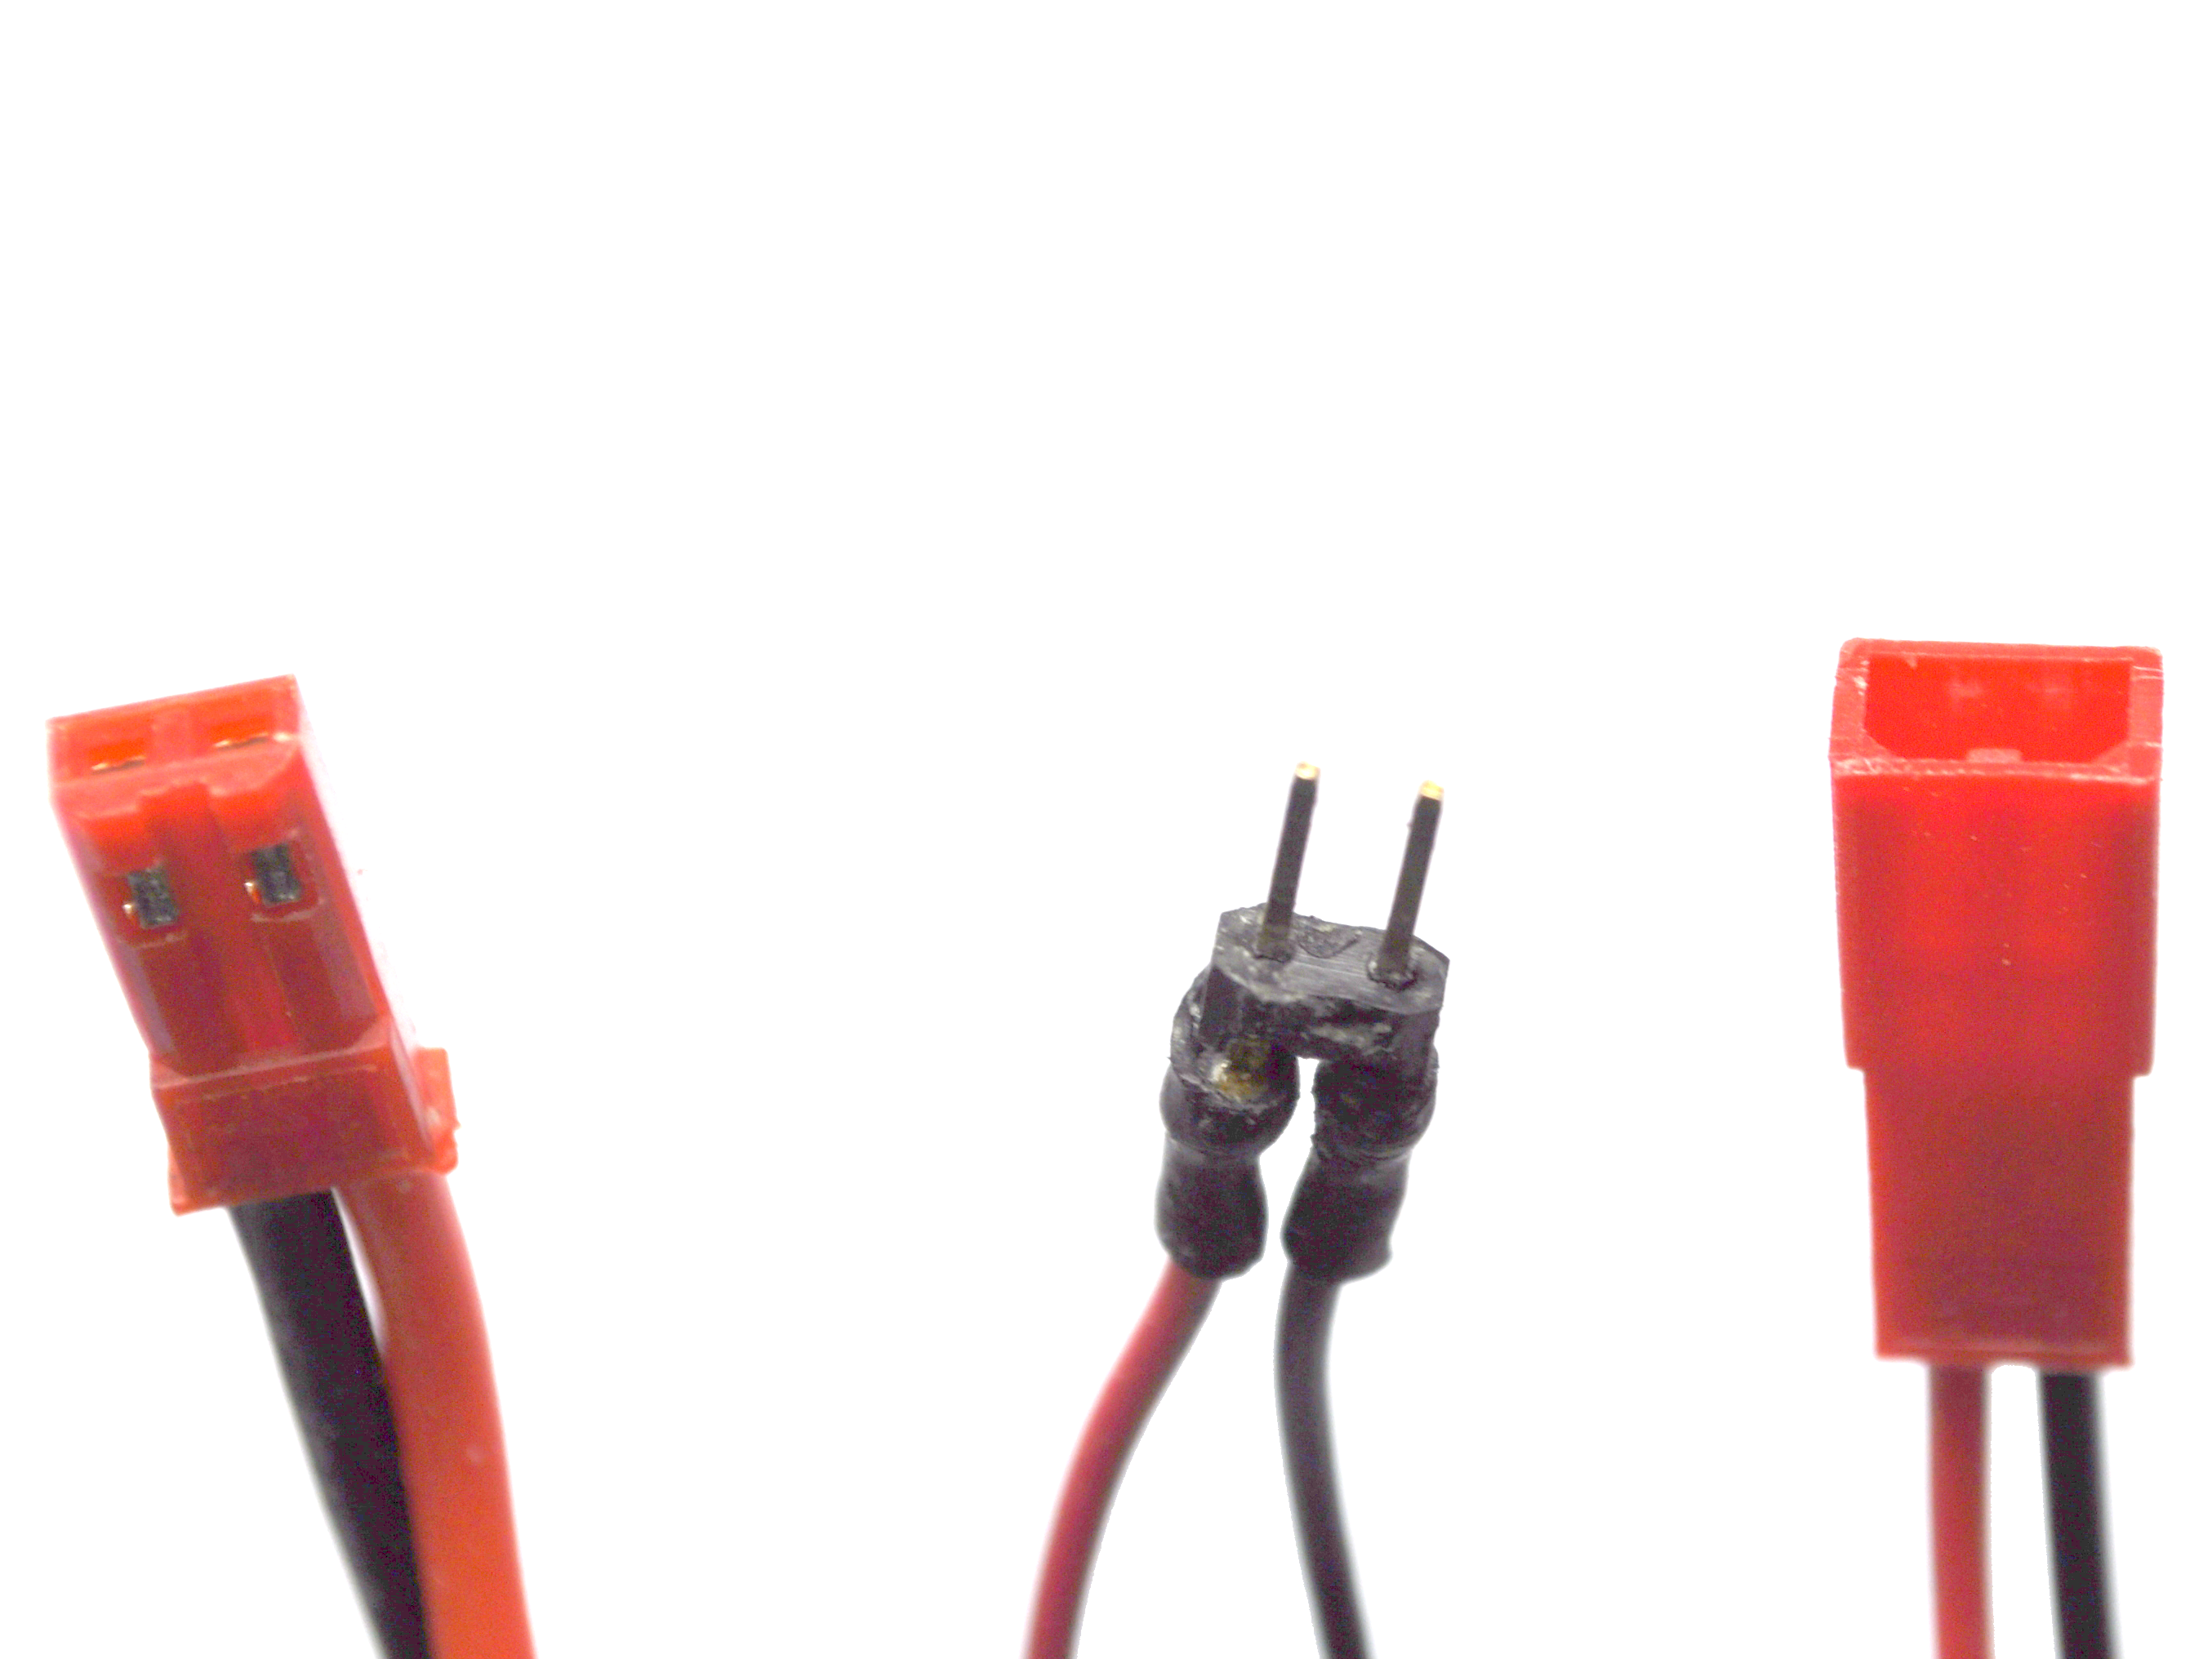
\includegraphics[width=\linewidth]{figures/battery-connectors.png}
		\caption{The power connectors}
		\label{fig:connectors}
		\medskip
		\small
		From left to right: female (battery), male unpolarized (old), male polarized (new)
	\end{minipage}
\end{figure}

\subsection{Electrical failure}

During one test of the hardware, the robot began to emit smoke from a then-unidentifiable location. The priority of course was to disconnect the battery as soon as possible to prevent a fireball, but even this proved difficult, with the melting power cables giving minor burns to a finger.

Methodical investigation followed, with the battery kept within its firesafe bag, and the entire system in a non-flammable enviroment. The process consisted of removing as much of the electronics as possible, and plugging in components one-by-one until a short was detected. This time, wire-cutters were used to break the battery connection quickly and safely when the issue arose.

The cause is shown in \cref{TODO}. On the bottom of the microcontroller board, there is a small metal stub fastening the pin headers to the top. These stubs were being used as resting points, with one pulled against a cable tie, and the other against a painted motor. With time, the paint wore through, causing a direct short between the Vin and GND pins - those connected directly to the battery.

The upshot here, of course, is that the short happened through a few components as possible, with damage found only in the wiring. To prevent this issue recurring, the metal screws connecting the microcontroller to the frame were replaced with nylon standoffs (\cref{fig:clearance}) - such that the board is now properly insulated from the frame, and furthermore has a far more rigid attachement.

As a precaution, a 3.15A fuse was inserted into the system, such that if a short happens in future, it does so without causing damage. The rating of the fuse was chosen to be in line with the stall current of the motors \ref{TODO}, making sure it did not exceed that of the 22AWG wires connecting it (roughly 5A).


% https://electronics.stackexchange.com/a/230164/1217
% http://batteryuniversity.com/learn/article/low_voltage_cut_off


\bib
\end{document}
